%Section start
% Изначальная миссия этого исследования, выходящего за рамки данной работы, анализировать эмоции собаки. Но для понимания даже базовых эмоций требуется уметь считывать базовые сигналы как поджатый, или наоборот, торчащий хвост. Либо оскал,  

Большинство людей интуитивно понимает основные значения телодвижений собаки и может определить, когда их собака счастлива, напугана или зла. Тем не менее язык тела человека и язык тела собаки очень различаются. Поза, выражение морды и телодвижения, которые мы интерпретируем как определенные эмоции, для вашей собаки могут означать нечто иное. 

По сути, язык тела собаки состоит из множества различных элементов, которые включают позу, выражение морды и телодвижения.

\subsection{Чтение коммуникационных сигналов тела собаки}

Язык тела собаки нельзя понять правильно, если при его интерпретации также не учитывать контекст и другие сигналы собаки. Например, оскал может означать радость, подчинение или агрессию — все зависит от остальных элементов языка тела.

\subsection{Положение тела собаки}

Анализ тела собаки в целом важен для определения эмоций собаки. Стоячее, вертикальное положение может означать доминирование или говорить об агрессии. Отодвинутое положение тела с весом, распределенным на зад собаки, говорит о страхе.\cite{Simpson1997}\cite{interpretation} Различие между активным и пассивным подчинением можно определить по позе собаки; активное подчинение проявляется в том, что собака держит тело низко на земле, в то время как пассивное подчинение проявляется в том, что собака лежит на земле с обнажённым брюшком.\cite{The_Domestic_Dog}.

Собака может изменить положение тела так, чтобы передняя часть тела находилась в прижатом положении, а передние лапы были ниже задних. Это может указывать на более высокий уровень агрессии, который может быть предвестником нападения. Если это положение сопровождается рычанием, морщинистым носом, расширенными зрачками, хвостом, заправленным под тело и между задними лапами, и приподнятой шерстью вдоль спины собаки, собака проявляет высокую агрессию и страх.\cite{speak_dog} Для сравнения, покорность может быть проявлена при опускании тела или при качении в сторону, обнажая подбородок.\cite{speak_dog}.


% на каждую секцию по фотке
\textbf{Расслабленное}. Расслабленность собаки можно определить, посмотрев на ее тело. Положение ее хвоста будет естественным, положение тела — непринужденным, а уши будут расслаблены или слегка направлены вверх. Собака не станет пристально смотреть или опускать глаза, а ее пасть будет расслаблена в уголках, челюсти сомкнуты или слегка приоткрыты.

\textbf{Возбужденное}. Собака быстро приближается к человеку или объекту, часто переходит на бег, прыжки и демонстрирует игривое настроение. При этом ее уши насторожены и подняты вверх, а хвост не успокаивается. Если пес чем-то особенно взволнован, он может также начать лаять или скулить.

\begin{figure}[ht] 
  \center
  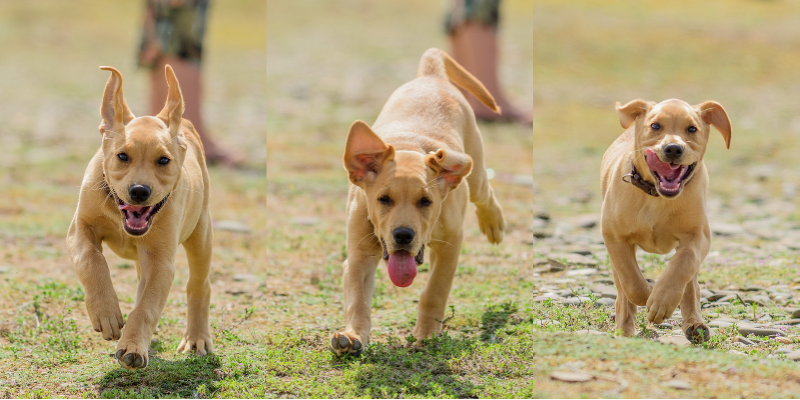
\includegraphics [width=\textwidth*2/3] {dog-run}
  \caption{Собака бежит в игривом настроении} 
  \label{img:dog-run}  
\end{figure}

\textbf{Напуганное}. Есть много способов, с помощью которых собака сообщает о страхе, и все они зависят от характера вашего питомца. Когда собаке страшно, она может нападать, прятаться и проявлять покорное поведение, а также искать утешения у своего хозяина. Большинство собак дрожит, прижимает тело к земле и зажимает хвост между ног.

\textbf{Игривое}. Собаку, которая хочет повеселиться, легко заметить. Типичная игривая стойка, когда передняя часть тела опущена на землю, а задние лапы выпрямлены, является недвусмысленным приглашением к игре как для хозяина, так и для другой собаки.

\textbf{Напряженное}. Если собака чувствует себя неуютно, она подаст об этом знак, напрягая и слегка опуская свое тело, а также направляя уши назад. У некоторых собак напряженная поза сопровождается зеванием или учащенным дыханием.

\textbf{Агрессивное}. Когда собака готовится к нападению, весь язык ее тела демонстрирует такое намерение. Агрессивные собаки имеют сосредоточенный или суженный взгляд, их тело напряжено, шерсть на затылке стоит дыбом, зубы обнажены в оскале, и можно услышать рычание. Тревожный лай и низкое рычание часто сопровождают агрессивное поведение собаки.